\iffalse
\let\negmedspace\undefined
\let\negthickspace\undefined
\documentclass[journal,12pt,onecolumn]{IEEEtran}
\usepackage{cite}
\usepackage{amsmath,amssymb,amsfonts,amsthm}
\usepackage{algorithmic}
\usepackage{graphicx}
\usepackage{textcomp}
\usepackage{xcolor}
\usepackage{txfonts}
\usepackage{listings}
\usepackage{enumitem}
\usepackage{mathtools}
\usepackage{gensymb}
\usepackage[breaklinks=true]{hyperref}
\usepackage{tkz-euclide} % loads  TikZ and tkz-base
\usepackage{listings}

\newcommand{\solution}{\noindent \textbf{Solution: }}
\newcommand{\cosec}{\,\text{cosec}\,}
\providecommand{\dec}[2]{\ensuremath{\overset{#1}{\underset{#2}{\gtrless}}}}
\newcommand{\myvec}[1]{\ensuremath{\begin{pmatrix}#1\end{pmatrix}}}
\newcommand{\mydet}[1]{\ensuremath{\begin{vmatrix}#1\end{vmatrix}}}
\newcommand{\myaugvec}[2]{\ensuremath{\begin{amatrix}{#1}#2\end{amatrix}}}
\providecommand{\rank}{\text{rank}}
\providecommand{\pr}[1]{\ensuremath{\Pr\left(#1\right)}}
\providecommand{\qfunc}[1]{\ensuremath{Q\left(#1\right)}}
\newcommand*{\permcomb}[4][0mu]{{{}^{#3}\mkern#1#2_{#4}}}
\newcommand*{\perm}[1][-3mu]{\permcomb[#1]{P}}
\newcommand*{\comb}[1][-1mu]{\permcomb[#1]{C}}
\providecommand{\qfunc}[1]{\ensuremath{Q\left(#1\right)}}
\providecommand{\gauss}[2]{\mathcal{N}\ensuremath{\left(#1,#2\right)}}
\providecommand{\diff}[2]{\ensuremath{\frac{d{#1}}{d{#2}}}}
\providecommand{\myceil}[1]{\left \lceil #1 \right \rceil }
\newcommand\figref{Fig.~\ref}
\newcommand\tabref{Table~\ref}
\newcommand{\sinc}{\,\text{sinc}\,}
\newcommand{\rect}{\,\text{rect}\,}


%\bibliographystyle{ieeetr}
\begin{document}
\providecommand{\pr}[1]{\ensuremath{\Pr\left(#1\right)}}
\providecommand{\prt}[2]{\ensuremath{p_{#1}^{\left(#2\right)} }}        % own macro for this question
\providecommand{\qfunc}[1]{\ensuremath{Q\left(#1\right)}}
\providecommand{\sbrak}[1]{\ensuremath{{}\left[#1\right]}}
\providecommand{\lsbrak}[1]{\ensuremath{{}\left[#1\right.}}
\providecommand{\rsbrak}[1]{\ensuremath{{}\left.#1\right]}}
\providecommand{\brak}[1]{\ensuremath{\left(#1\right)}}
\providecommand{\lbrak}[1]{\ensuremath{\left(#1\right.}}
\providecommand{\rbrak}[1]{\ensuremath{\left.#1\right)}}
\providecommand{\cbrak}[1]{\ensuremath{\left\{#1\right\}}}
\providecommand{\lcbrak}[1]{\ensuremath{\left\{#1\right.}}
\providecommand{\rcbrak}[1]{\ensuremath{\left.#1\right\}}}
\newcommand{\sgn}{\mathop{\mathrm{sgn}}}
\providecommand{\abs}[1]{\left\vert#1\right\vert}
\providecommand{\res}[1]{\Res\displaylimits_{#1}} 
\providecommand{\norm}[1]{\left\lVert#1\right\rVert}
%\providecommand{\norm}[1]{\lVert#1\rVert}
\providecommand{\mtx}[1]{\mathbf{#1}}
\providecommand{\mean}[1]{E\left[ #1 \right]}
\providecommand{\cond}[2]{#1\middle|#2}
\providecommand{\fourier}{\overset{\mathcal{F}}{ \rightleftharpoons}}
\newenvironment{amatrix}[1]{%
  \left(\begin{array}{@{}*{#1}{c}|c@{}}
}{%
  \end{array}\right)
}
%\providecommand{\hilbert}{\overset{\mathcal{H}}{ \rightleftharpoons}}
%\providecommand{\system}{\overset{\mathcal{H}}{ \longleftrightarrow}}
%\newcommand{\solution}[2]{\textbf{Solution:}{#1}}
%%
%%\newcommand{\solution}[2]{\textbf{Solution:}{#1}}
%\newcommand{\solution}{\noindent \textbf{Solution: }}
%\newcommand{\cosec}{\,\text{cosec}\,}
%\numberwithin{equation}{section}
%\numberwithin{equation}{subsection}
%\numberwithin{problem}{section}
%\numberwithin{definition}{section}
%\makeatletter
%\@addtoreset{figure}{problem}
%\makeatother
%\let\StandardTheFigure\thefigure
\let\vec\mathbf
\bibliographystyle{IEEEtran}

\vspace{3cm}

\bigskip

\renewcommand{\thefigure}{\theenumi}
\renewcommand{\thetable}{\theenumi}
%\renewcommand{\theequation}{\theenumi}

\textbf{Question }\\
A box has 100 pens of which 10 are defective . What is the probability that out of a sample of 5 pens drawn one by one with replacement at most one is defective?\\
(A)$\left(\frac{9}{10}\right)^5$\\
(B)$\frac{1}{2}\left(\frac{9}{5}\right)^4$\\
(C)$\frac{1}{2}\left(\frac{9}{10}\right)^5$\\
(D)$\frac{1}{2}\left(\frac{9}{5}\right)^4+\left(\frac{9}{10}\right)^5 $\\
\solution\\
\fi
\begin{table}[!ht]
\centering
\begin{tabular}{|l|c|r|}
    \hline
    Parameter & Values & Description\\
    \hline
    $n$ & 5 & Number of defective pens \\
    \hline
    $p$ & 0.1 &probability of drawing a defective pen \\
    \hline
    $\mu$ & 0.5 & np \\
    \hline
    $\sigma $ & 0.671 & $\sqrt{np(1-p)} $\\
    \hline
    $ X $ &  &  Defective pens \\
    \hline
\end{tabular}
\label{tab:gaussian/9/3/33}
\end{table}

\textbf{Using Binomial}\\
Given,\\
Probability of drawing a defective pen = $\frac{1}{10}$\\
Probability of drawing a non-defective pen = $\frac{9}{10}$\\
Let,\\
Probability of drawing atmost one pen out of 5 defective with replacement = $\pr{X \le 1}$
\begin{align}
\pr{X \le 1} = p_X\brak{0} + p_X\brak{1}\\
\implies \pr{X \le 1} = \binom{5}{0}\left(\frac{9}{10}\right)^5 + \binom{5}{1}\left(\frac{9}{10}\right)^4\left(\frac{1}{10}\right)\\
= \left(\frac{9}{10}\right)^5 + 5\left(\frac{9}{10}\right)^4\left(\frac{1}{10}\right)\\
= \left(\frac{9}{10}\right)^5 + \frac{1}{2}\left(\frac{9}{10}\right)^4\\
= 0.91854
\end{align}

\textbf{Gaussian}
\begin{align}
Y \sim \gauss{\mu}{\sigma^2}
\end{align}
CDF of Y is
\begin{align}
F_{Y}\brak{y} &= \pr{Y \leq y}
\end{align}
We know that 
\begin{align}
\qfunc{x} &= \pr{X > x}, x > 0, X \sim N(0,1)\\
\qfunc{-x} &= \pr{X > -x}, x < 0, X \sim N(0,1)\\
&= 1 - \qfunc{x}
\end{align}
Hence,\\
CDF :
\begin{align}
F_Y\brak{y} &= \begin{cases}
                 1 - \qfunc{\frac{y - \mu}{\sigma}},& \text{if $y > \mu$}\\
                 1 - \qfunc{\frac{y - \mu}{\sigma}} = \qfunc{\frac{\mu - y}{\sigma}},& \text{if $y < \mu$}
               \end{cases}
\end{align}
\begin{align}
F_Y\brak{1} &= \pr{Y \leq 1}\\
&= 1 - \qfunc{\frac{1 - 0.5}{\sqrt{0.671}}}\\
&= 1 - \qfunc{\frac{0.5}{0.819}}\\
&= 1 - \qfunc{0.6104}\\
&= 0.729198876
\end{align}
\begin{figure}[!ht]
\centering
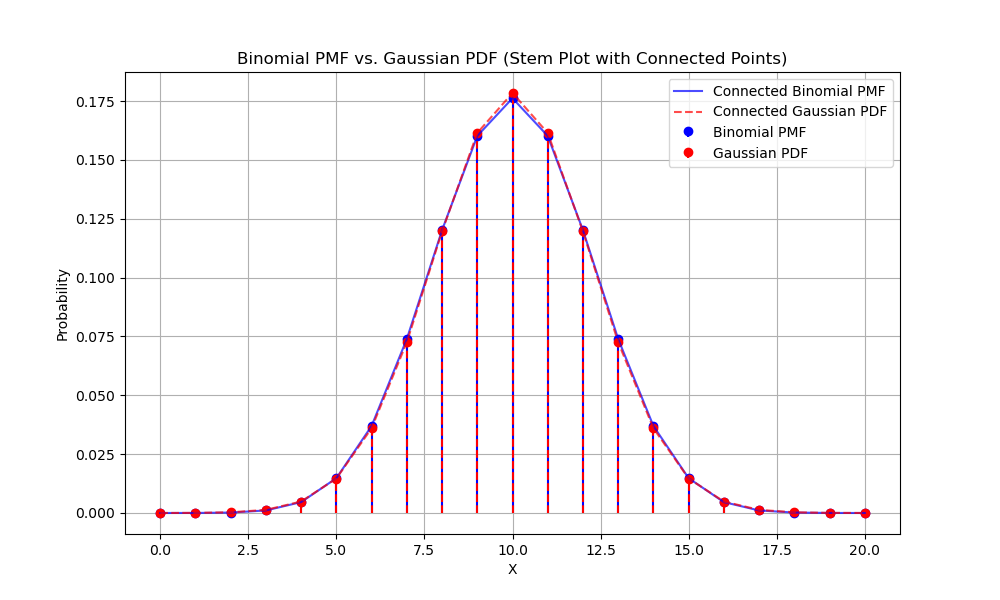
\includegraphics[width=\columnwidth]{ncert/9/3/33/figs/Fig1.png}
\caption{pmf of binomial and pdf of Gaussian of X and Y marked balls}
\label{fig:gaussian/9/3/33/}
\end{figure}

